\documentclass[11pt,a4paper]{article}

\usepackage[T1]{fontenc}
\usepackage[margin=1in]{geometry}
\usepackage{amsmath}
\usepackage{amssymb}
\usepackage{array}
\usepackage{booktabs}
\usepackage{xcolor}
\usepackage{tikz}
\usetikzlibrary{arrows.meta,positioning,calc,fit}

\title{ELEC5803 HLS Exam Study\\Step-by-Step Solution to Question 3}
\author{}
\date{}

\tikzset{
  >={Latex[length=2mm]},
  neuron/.style={draw, circle, fill=blue!12, minimum size=8mm, inner sep=0pt},
  reg/.style={draw, rounded corners, fill=blue!6, minimum width=1.5cm, minimum height=0.8cm, align=center},
  fu/.style={draw, rounded corners, fill=green!8, minimum width=2.5cm, minimum height=0.9cm, align=center},
  ctrl/.style={draw, rounded corners, fill=orange!10, minimum width=2.5cm, minimum height=0.9cm, align=center},
  small/.style={draw, rounded corners, minimum width=1.6cm, minimum height=0.7cm, align=center},
}

\begin{document}
\maketitle

\section*{Course-slide basis}
This solution uses the same HLS ideas emphasized in:
\begin{itemize}
  \item \textbf{Slides 5}: operation scheduling and resource-constrained scheduling.
  \item \textbf{Slides 6}: datapath allocation, bus-oriented interconnection, and hardware sharing.
\end{itemize}

\section*{1. Interpreting the neural network}
The figure shows three computational stages of neurons:
\[
(N_1,N_2,N_3)\rightarrow (N_4,N_5,N_6)\rightarrow (N_7,N_8,N_9)\rightarrow (O_1,O_2,O_3).
\]
For a representative neuron such as $N_4$, the inputs are the outputs of $N_1$, $N_2$, and $N_3$:
\[
s_4 = W_{14}N_1 + W_{24}N_2 + W_{34}N_3
\]
and the neuron output is
\[
N_4=f(s_4),\qquad
f(x)=
\begin{cases}
1,&x\ge 0\\
0,&x<0.
\end{cases}
\]

\begin{figure}[h!]
\centering
\resizebox{\textwidth}{!}{%
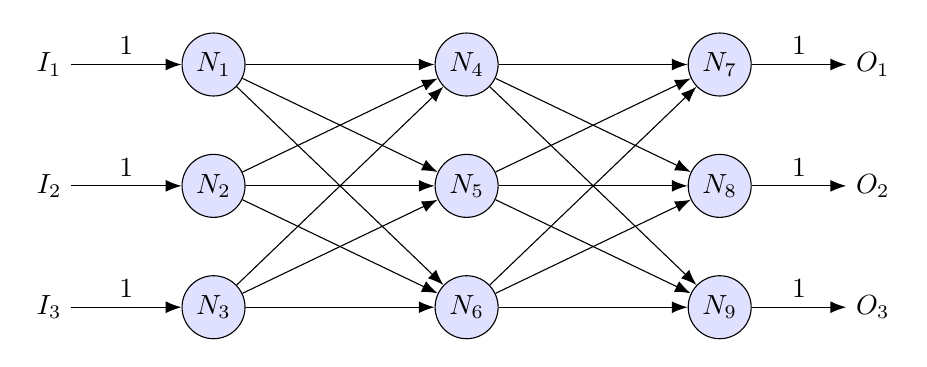
\begin{tikzpicture}[node distance=8mm and 12mm]
  \node (i1) {$I_1$};
  \node[below=10mm of i1] (i2) {$I_2$};
  \node[below=10mm of i2] (i3) {$I_3$};

  \node[neuron, right=14mm of i1] (n1) {$N_1$};
  \node[neuron, right=14mm of i2] (n2) {$N_2$};
  \node[neuron, right=14mm of i3] (n3) {$N_3$};

  \node[neuron, right=24mm of n1] (n4) {$N_4$};
  \node[neuron, right=24mm of n2] (n5) {$N_5$};
  \node[neuron, right=24mm of n3] (n6) {$N_6$};

  \node[neuron, right=24mm of n4] (n7) {$N_7$};
  \node[neuron, right=24mm of n5] (n8) {$N_8$};
  \node[neuron, right=24mm of n6] (n9) {$N_9$};

  \node[right=12mm of n7] (o1) {$O_1$};
  \node[right=12mm of n8] (o2) {$O_2$};
  \node[right=12mm of n9] (o3) {$O_3$};

  \draw[->] (i1) -- node[above] {$1$} (n1);
  \draw[->] (i2) -- node[above] {$1$} (n2);
  \draw[->] (i3) -- node[above] {$1$} (n3);

  \foreach \a in {1,2,3}{
    \foreach \b/\c in {4/n4,5/n5,6/n6}{
      \draw[->] (n\a) -- (\c);
    }
  }
  \foreach \a/\na in {4/n4,5/n5,6/n6}{
    \foreach \b/\c in {7/n7,8/n8,9/n9}{
      \draw[->] (\na) -- (\c);
    }
  }
  \draw[->] (n7) -- node[above] {$1$} (o1);
  \draw[->] (n8) -- node[above] {$1$} (o2);
  \draw[->] (n9) -- node[above] {$1$} (o3);
\end{tikzpicture}%
}
\caption{Native-LaTeX redraw of the Q3 network.}
\end{figure}

\section*{2. Part (a): scheduling diagram for one neuron}
\subsection*{2.1 Operations of neuron $N_4$}
For one neuron with three inputs, define:
\[
\begin{aligned}
m_1 &= W_{14}N_1,\\
m_2 &= W_{24}N_2,\\
m_3 &= W_{34}N_3,\\
a_1 &= m_1+m_2,\\
a_2 &= a_1+m_3,\\
N_4 &= f(a_2).
\end{aligned}
\]
So the computation graph is:
\[
\{m_1,m_2,m_3\}\rightarrow a_1\rightarrow a_2\rightarrow f.
\]

\subsection*{2.2 ASAP-style schedule}
With unconstrained resources, the natural schedule is:
\begin{center}
\begin{tabular}{lcccc}
\toprule
Operation & CS1 & CS2 & CS3 & CS4 \\
\midrule
$m_1=W_{14}N_1$ & $\bullet$ & & & \\
$m_2=W_{24}N_2$ & $\bullet$ & & & \\
$m_3=W_{34}N_3$ & $\bullet$ & & & \\
$a_1=m_1+m_2$ & & $\bullet$ & & \\
$a_2=a_1+m_3$ & & & $\bullet$ & \\
$N_4=f(a_2)$ & & & & $\bullet$ \\
\bottomrule
\end{tabular}
\end{center}

\begin{figure}[h!]
\centering
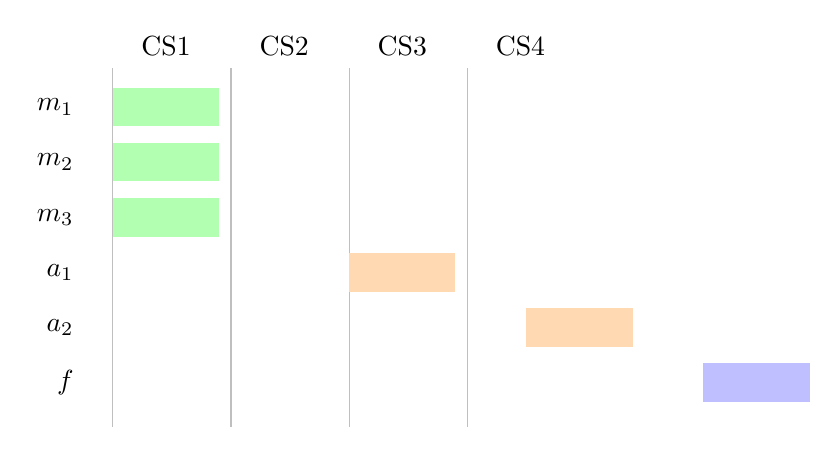
\begin{tikzpicture}[x=1.5cm,y=0.7cm]
  \foreach \x/\lab in {1/CS1,2/CS2,3/CS3,4/CS4}{
    \node at (\x,1.1) {\lab};
    \draw[gray!50] (\x-0.45,-5.8) -- (\x-0.45,0.7);
  }
  \foreach \y/\lab in {0/$m_1$, -1/$m_2$, -2/$m_3$, -3/$a_1$, -4/$a_2$, -5/$f$}{
    \node[left] at (0.3,\y) {\lab};
  }
  \fill[green!30] (0.55,-0.35) rectangle (1.45,0.35);
  \fill[green!30] (0.55,-1.35) rectangle (1.45,-0.65);
  \fill[green!30] (0.55,-2.35) rectangle (1.45,-1.65);
  \fill[orange!30] (2.55,-3.35) rectangle (3.45,-2.65);
  \fill[orange!30] (4.05,-4.35) rectangle (4.95,-3.65);
  \fill[blue!25] (5.55,-5.35) rectangle (6.45,-4.65);
\end{tikzpicture}
\caption{Scheduling diagram for a single neuron under unlimited resources.}
\end{figure}

\subsection*{2.3 Interpretation}
This is exactly the kind of precedence-based scheduling discussed in Slides 5:
\begin{itemize}
  \item the three multiplications are mutually independent,
  \item the first addition must wait for $m_1$ and $m_2$,
  \item the second addition must wait for $a_1$ and $m_3$,
  \item the activation function waits for the final sum.
\end{itemize}

\section*{3. Part (b): single-neuron hardware with at most two adders and two multipliers using a single bus}
\subsection*{3.1 Resource constraint}
We are allowed:
\begin{itemize}
  \item at most 2 multipliers,
  \item at most 2 adders,
  \item a single shared bus.
\end{itemize}

The datapath for one neuron can therefore contain:
\begin{itemize}
  \item an input/weight memory or register file,
  \item one shared single bus,
  \item two multiplier input register pairs,
  \item two multipliers,
  \item one accumulator adder for the partial sums,
  \item one threshold unit implementing the Heaviside function,
  \item a controller.
\end{itemize}

\subsection*{3.2 Single-bus schedule}
Because the bus is shared, operand transfers must be serialized. A clean schedule is:
\begin{center}
\begin{tabular}{cl}
\toprule
Step & Micro-operation \\
\midrule
1 & Bus $\leftarrow N_1$, load multiplier-1 operand register \\
2 & Bus $\leftarrow W_{14}$, load multiplier-1 weight register \\
3 & Bus $\leftarrow N_2$, load multiplier-2 operand register \\
4 & Bus $\leftarrow W_{24}$, load multiplier-2 weight register \\
5 & In parallel: $m_1=W_{14}N_1$, $m_2=W_{24}N_2$ \\
6 & $s_{12}=m_1+m_2$ \\
7 & Bus $\leftarrow N_3$, load multiplier-1 operand register \\
8 & Bus $\leftarrow W_{34}$, load multiplier-1 weight register \\
9 & $m_3=W_{34}N_3$ \\
10 & $s=s_{12}+m_3$ \\
11 & $N_4=f(s)$ \\
\bottomrule
\end{tabular}
\end{center}

\noindent
Only one adder is actually required for the accumulation chain. The second available adder does not reduce the latency here because the second addition depends on the first partial sum.

\subsection*{3.3 Hardware schematic}
\begin{figure}[h!]
\centering
\resizebox{\textwidth}{!}{%
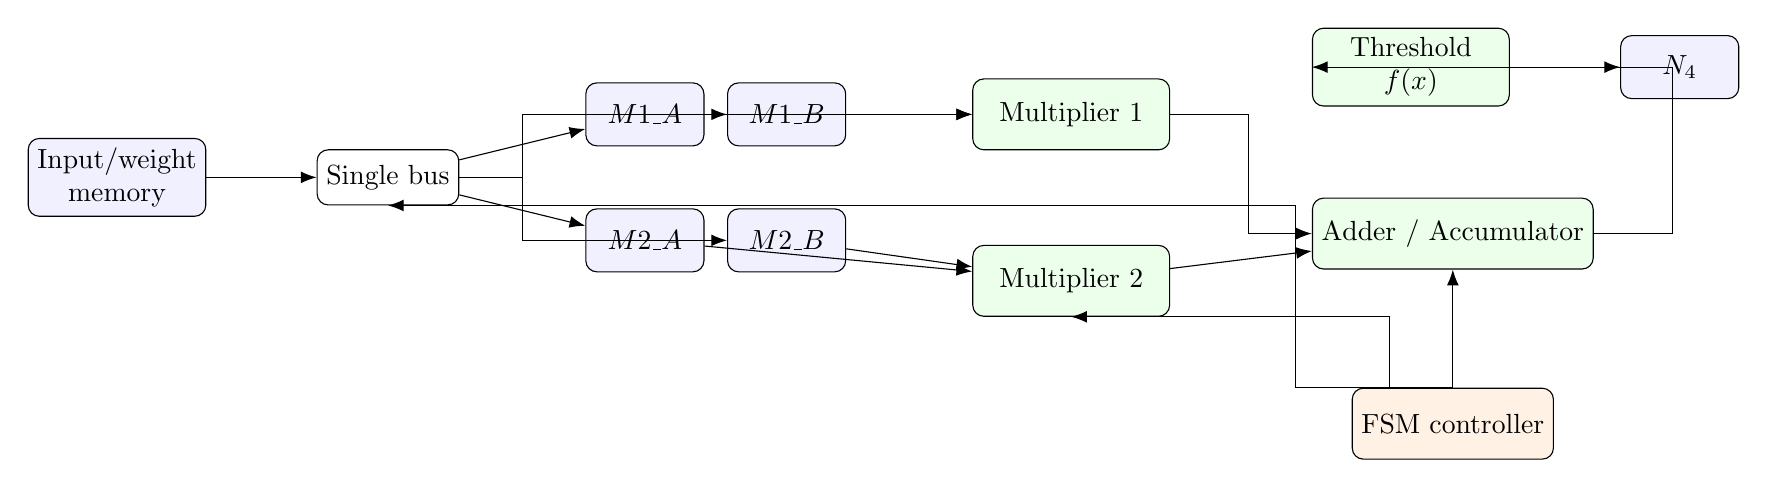
\begin{tikzpicture}[node distance=8mm and 10mm]
  \node[reg] (mem) {Input/weight\\memory};
  \node[small, right=14mm of mem] (bus) {Single bus};

  \node[reg, right=16mm of bus, yshift=8mm] (m1a) {$M1\_A$};
  \node[reg, right=16mm of bus, yshift=-8mm] (m2a) {$M2\_A$};
  \node[reg, right=34mm of bus, yshift=8mm] (m1b) {$M1\_B$};
  \node[reg, right=34mm of bus, yshift=-8mm] (m2b) {$M2\_B$};

  \node[fu, right=16mm of m1b] (mul1) {Multiplier 1};
  \node[fu, below=12mm of mul1] (mul2) {Multiplier 2};
  \node[fu, right=18mm of mul2, yshift=6mm] (add) {Adder / Accumulator};
  \node[fu, right=18mm of mul1, yshift=6mm] (thr) {Threshold\\$f(x)$};
  \node[reg, right=14mm of thr] (out) {$N_4$};
  \node[ctrl, below=15mm of add] (ctrl) {FSM controller};

  \draw[->] (mem) -- (bus);
  \draw[->] (bus) -- (m1a);
  \draw[->] (bus) -- (m2a);
  \draw[->] (bus.east) -- ++(8mm,0) |- (m1b.west);
  \draw[->] (bus.east) -- ++(8mm,0) |- (m2b.west);

  \draw[->] (m1a) -- (mul1);
  \draw[->] (m1b) -- (mul1);
  \draw[->] (m2a) -- (mul2);
  \draw[->] (m2b) -- (mul2);

  \draw[->] (mul1.east) -- ++(10mm,0) |- (add.west);
  \draw[->] (mul2) -- (add);
  \draw[->] (add.east) -- ++(10mm,0) |- (thr.west);
  \draw[->] (thr) -- (out);

  \draw[->] (ctrl.north) -- (add.south);
  \draw[->] (ctrl.north) -- ++(-8mm,0) |- (mul2.south);
  \draw[->] (ctrl.north) -- ++(-20mm,0) |- (bus.south);
\end{tikzpicture}%
}
\caption{Single-neuron hardware under the given resource constraint and a single-bus datapath.}
\end{figure}

\subsection*{3.4 Why this satisfies the question}
This design matches the HLS allocation ideas from Slides 6:
\begin{itemize}
  \item arithmetic resources are bounded,
  \item the bus is a shared interconnection unit,
  \item the controller sequences operand transfers and functional-unit use,
  \item the datapath is a small FSMD-style realization of one neuron.
\end{itemize}

\clearpage
\section*{4. Part (c): total inference delay using the neuron design and a flexible multi-bus network}
\subsection*{4.1 Assumptions}
To keep the symbolic delay expression consistent with the question, use the following assumptions:
\begin{itemize}
  \item memory access delay is $T_{\text{MEM}}$,
  \item multiplication delay is $T_{\text{MUL}}$,
  \item addition delay is $T_{\text{ADD}}$,
  \item the threshold comparison is small and is not parameterized in the question, so it is neglected,
  \item the edges marked with weight 1 at the input and output are treated as direct connections rather than full multiply operations.
\end{itemize}

\subsection*{4.2 Delay of one 3-input neuron with two multipliers}
With a \emph{flexible multi-bus} implementation, bus conflicts are removed, so the neuron can use both multipliers efficiently.

One good schedule for a neuron is:
\begin{center}
\begin{tabular}{clc}
\toprule
Stage & Operations & Delay \\
\midrule
1 & Fetch two input-weight pairs and compute $m_1,m_2$ in parallel & $T_{\text{MEM}}+T_{\text{MUL}}$ \\
2 & Fetch third pair, compute $m_3$ while also computing $a_1=m_1+m_2$ & $\max(T_{\text{ADD}},\,T_{\text{MEM}}+T_{\text{MUL}})$ \\
3 & Compute $a_2=a_1+m_3$ & $T_{\text{ADD}}$ \\
\bottomrule
\end{tabular}
\end{center}

Therefore, the latency of one 3-input neuron is
\[
\boxed{
T_{\text{neuron}}
=
(T_{\text{MEM}}+T_{\text{MUL}})
\;+\;
\max(T_{\text{ADD}},\,T_{\text{MEM}}+T_{\text{MUL}})
\;+\;
T_{\text{ADD}}.
}
\]

\subsection*{4.3 Layer-by-layer inference}
In the given network:
\begin{itemize}
  \item neurons $N_4,N_5,N_6$ form one 3-neuron layer,
  \item neurons $N_7,N_8,N_9$ form the next 3-neuron layer,
  \item all neurons in the same layer are independent and can therefore be evaluated in parallel in a multi-bus implementation.
\end{itemize}

Hence:
\begin{itemize}
  \item delay of layer $(N_4,N_5,N_6)$ is $T_{\text{neuron}}$,
  \item delay of layer $(N_7,N_8,N_9)$ is also $T_{\text{neuron}}$.
\end{itemize}

So the total inference delay is
\[
\boxed{
T_{\text{inf}}=2\,T_{\text{neuron}}.
}
\]
Substituting the neuron latency:
\[
\boxed{
T_{\text{inf}}
=
2\Big[
(T_{\text{MEM}}+T_{\text{MUL}})
\max(T_{\text{ADD}},\,T_{\text{MEM}}+T_{\text{MUL}})
T_{\text{ADD}}
\Big].
}
\]

\subsection*{4.4 Common simplification}
In most practical datapaths,
\[
T_{\text{MEM}}+T_{\text{MUL}} \ge T_{\text{ADD}}.
\]
Then the expression simplifies to:
\[
\boxed{
T_{\text{inf}} = 2\,(2T_{\text{MEM}}+2T_{\text{MUL}}+T_{\text{ADD}}).
}
\]

\subsection*{4.5 Network schematic for inference}
\begin{figure}[h!]
\centering
\resizebox{\textwidth}{!}{%
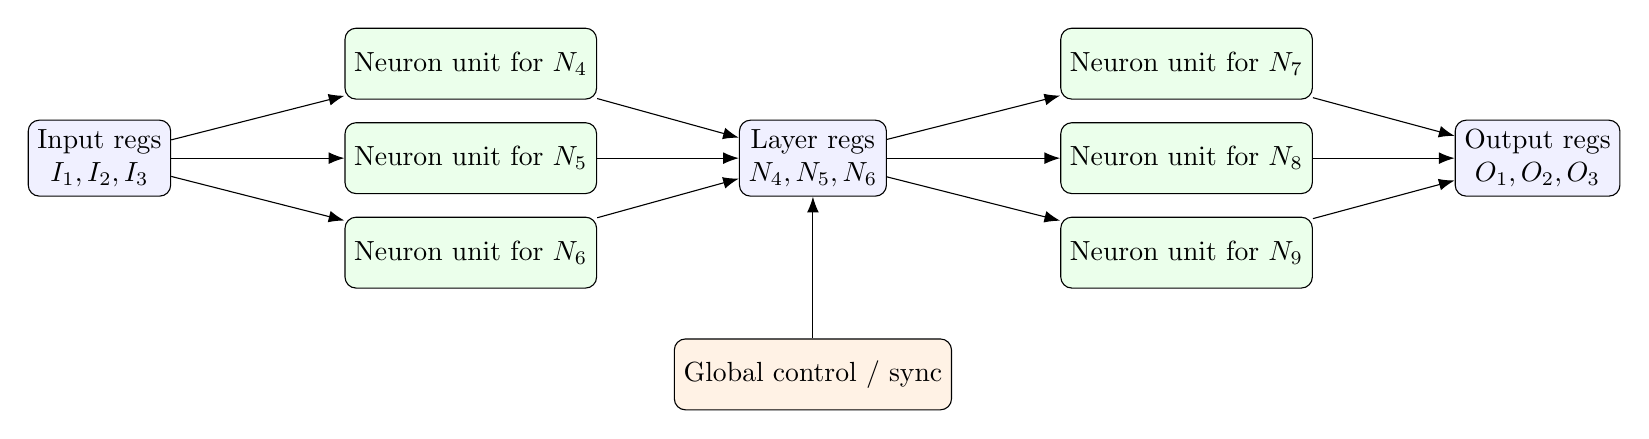
\begin{tikzpicture}[node distance=10mm and 14mm]
  \node[reg] (in) {Input regs\\$I_1,I_2,I_3$};

  \node[fu, right=22mm of in, yshift=12mm] (u4) {Neuron unit for $N_4$};
  \node[fu, right=22mm of in] (u5) {Neuron unit for $N_5$};
  \node[fu, right=22mm of in, yshift=-12mm] (u6) {Neuron unit for $N_6$};

  \node[reg, right=18mm of u5] (mid) {Layer regs\\$N_4,N_5,N_6$};

  \node[fu, right=22mm of mid, yshift=12mm] (u7) {Neuron unit for $N_7$};
  \node[fu, right=22mm of mid] (u8) {Neuron unit for $N_8$};
  \node[fu, right=22mm of mid, yshift=-12mm] (u9) {Neuron unit for $N_9$};

  \node[reg, right=18mm of u8] (out) {Output regs\\$O_1,O_2,O_3$};
  \node[ctrl, below=18mm of mid] (ctrl) {Global control / sync};

  \draw[->] (in) -- (u4);
  \draw[->] (in) -- (u5);
  \draw[->] (in) -- (u6);
  \draw[->] (u4) -- (mid);
  \draw[->] (u5) -- (mid);
  \draw[->] (u6) -- (mid);
  \draw[->] (mid) -- (u7);
  \draw[->] (mid) -- (u8);
  \draw[->] (mid) -- (u9);
  \draw[->] (u7) -- (out);
  \draw[->] (u8) -- (out);
  \draw[->] (u9) -- (out);
  \draw[->] (ctrl.north) -- (mid.south);
\end{tikzpicture}%
}
\caption{Flexible multi-bus network implementation: all three neurons in a layer execute in parallel, and the next layer starts after the layer registers are updated.}
\end{figure}

\section*{5. Final exam-style answers}
\subsection*{(a) Scheduling diagram}
For one neuron such as $N_4$:
\begin{itemize}
  \item CS1: three multiplications,
  \item CS2: first addition,
  \item CS3: second addition,
  \item CS4: Heaviside activation.
\end{itemize}

\subsection*{(b) Single-bus neuron hardware}
Use a small FSMD datapath with:
\begin{itemize}
  \item one input/weight memory,
  \item one shared bus,
  \item two multipliers,
  \item one accumulator adder,
  \item one threshold unit,
  \item one controller.
\end{itemize}
Serialized bus transfers load the two multipliers, then the partial sums are accumulated.

\subsection*{(c) Total inference delay}
Using a flexible multi-bus network so that all neurons in a layer run in parallel:
\[
\boxed{
T_{\text{inf}}
=
2\Big[
(T_{\text{MEM}}+T_{\text{MUL}})
\max(T_{\text{ADD}},\,T_{\text{MEM}}+T_{\text{MUL}})
T_{\text{ADD}}
\Big].
}
\]
If $T_{\text{MEM}}+T_{\text{MUL}}\ge T_{\text{ADD}}$, then
\[
\boxed{
T_{\text{inf}} = 2\,(2T_{\text{MEM}}+2T_{\text{MUL}}+T_{\text{ADD}}).
}
\]

\end{document}
